\documentclass[11pt]{article}

\usepackage[margin=1in]{geometry}
\usepackage[T1]{fontenc}
\usepackage{lmodern}
\usepackage{microtype}
\usepackage{amsmath}
\usepackage{booktabs}
\usepackage{graphicx}
\usepackage{xcolor}
\usepackage[numbers,sort&compress]{natbib}
\usepackage[hidelinks]{hyperref}

\graphicspath{{figs/}}
\newcommand{\todo}[1]{\textcolor{red}{[TODO: #1]}}
\newcommand{\ci}[2]{\,[#1,\,#2]}

\title{Scan or Search?\\[2pt]
\large Exhaustive LLM Classification versus Agentic Search for Find-All Queries}
\author{Ayesha Shafique \and Nabanita Bag \and Nida Tanveer\\[2pt]
\normalsize CS 839, University of Wisconsin--Madison}
\date{December 2026}

\begin{document}
\maketitle

\begin{abstract}
Some queries ask for \emph{every} document that matches a description: all
reports about a product defect, all papers on a method, all emails about a
deal. An LLM can answer such a query in two ways. It can \emph{search}: an
agent issues retrieval queries, reads the results and decides when to stop.
Or it can \emph{scan}: a classifier asks ``does this document match?'' of
every document, in large GPU batches. We compare the two on corpora where the
full answer set is known, using the same model, Qwen2.5-7B-Instruct, for both
on one H200 GPU. We express the cost of an agent as an \emph{exchange rate}:
one agent step costs as much GPU time as 78 scan decisions when queries run
one at a time, and 11 when about 50 queries share the GPU. At equal time per
query, a scan that visits documents in embedding order finds three times as
many answers as the agent at 10,000 documents (recall 0.26 against 0.09).
Batching makes the agent as cheap as the scan, but not more complete: its
recall stays at 0.09. Choosing how far down the ranking to scan for each query
(adaptive $k$) does not beat a fixed depth at equal cost, and an oracle bound
shows there is little to gain. Finally, replacing the zero-shot classifier
with a purpose-built open decision model, Kev-9B, raises the scan's recall
from 0.31 to 0.78 at the default threshold, and in the agent's own time the
scan reaches recall 0.48 one query at a time and 0.71 when queries share a
pass over the documents. \todo{one sentence on JEV-9B.}
\end{abstract}

% ---------------------------------------------------------------------------
\section{Introduction}

Retrieval systems are usually judged on the top of a ranking. Many real tasks
instead need the whole answer set: legal discovery, systematic reviews,
compliance audits and dataset curation all ask for \emph{all} matching
documents, and a missed document is a real cost. We call these
\emph{find-all queries}.

LLMs offer two ways to answer them. An \emph{agent} wraps a retriever in a
reasoning loop~\cite{yao2023react}: it writes a search query, reads the
results, keeps the matches and searches again until it decides it is done.
It reads only a small part of the corpus, so it is cheap, but it cannot know
what it never retrieved. A \emph{scan} asks a yes/no question of every
document. Each decision is one short prefill with no decoding, and the
decisions are independent, so they batch well on a GPU~\cite{kwon2023vllm}.
It is complete by construction but costs $O(N)$ model calls. Hosted decision
models such as TypeSafe's Jev~\cite{typesafe_jev} are built for the second
pattern, and open reproductions such as Kev~\cite{kev} and
JEV-9B~\cite{jev9b} now make it possible to study it.

This project asks: \emph{for a find-all query, when is it better to classify
every document in parallel than to let an LLM agent search?} Our
contributions are:
\begin{enumerate}
  \item A measured comparison of scan and agent on corpora with complete
  answer sets, with the same model as classifier and agent, so the
  comparison isolates the execution strategy (\S\ref{sec:headline}).
  \item The \emph{exchange rate}: how many scan decisions one agent step buys
  on the same GPU, and how batching agents changes it
  (\S\ref{sec:exchange}).
  \item An equal-time comparison showing that a scan in embedding order beats
  the agent one query at a time, and that batched agents only tie it, at the
  agent's low recall (\S\ref{sec:equaltime}).
  \item A negative result for adaptive $k$, framed as cost-based access-path
  selection, with an oracle bound on what any such rule could gain
  (\S\ref{sec:adaptive}).
  \item Evidence that most of the scan's recall gap comes from using a
  zero-shot model: open, purpose-built decision models raise recall sharply
  and remove the need for threshold tuning (\S\ref{sec:decision}).
\end{enumerate}

% ---------------------------------------------------------------------------
\section{Related work}

\paragraph{Ranked list truncation.}
Deciding how far down a ranking to go is studied as ranked list truncation.
Choppy~\cite{bahri2020choppy} and AttnCut~\cite{wu2021attncut} learn a cut-off
from the scores of a ranked list to optimise a user metric such as F1. Meng
et al.~\cite{meng2024rlt} reproduce eight such methods for LLM re-ranking and
find that supervised truncation shows no clear advantage over a fixed
re-ranking depth; with a strong first-stage retriever, a fixed depth already
gives a good effectiveness--efficiency trade-off. Adaptive-$k$
\cite{taguchi2025adaptivek} picks the number of passages for RAG from the
shape of the similarity distribution. Our adaptive-$k$ rules
(\S\ref{sec:adaptive}) take ideas from both, and our result agrees with Meng
et al.

\paragraph{Stopping rules for high-recall review.}
Technology-assisted review (TAR) faces the same question in a human loop:
when has review found enough? Cormack and Grossman~\cite{cormack2016tar}
propose the knee and target methods; Yang et al.~\cite{yang2021stopping}
derive stopping rules from survey-sampling estimates of recall. Our
\emph{yield} rule is a simple knee-style rule, and our \emph{sample} rule
estimates the answer size from a random sample, as the target method does.

\paragraph{Semantic filtering in data systems.}
LOTUS~\cite{patel2024lotus} defines semantic operators, including
\texttt{sem\_filter}, whose reference (``gold'') algorithm is exactly our scan:
one batched LLM call per tuple. Its optimiser runs a cheap proxy model, learns
two thresholds from a labelled sample so that precision and recall targets
hold with high probability, and sends only the uncertain band to the large
model. Kim et al.~\cite{kim2026semfilter} unify such cascades and combine
clustering, an online proxy and shared oracle calls, reporting 1.6--2.0$\times$
speedups at a 90\% accuracy target. These systems make the scan cheaper; we
instead ask when the scan is worth running at all compared with an agent, and
we deliberately leave cascades out of scope.

\paragraph{Decision models.}
Jev~\cite{typesafe_jev} is a hosted model that answers typed questions (yes/no,
multiple choice, scores) about a given state in one prefill pass, returning a
probability distribution instead of text. Kev~\cite{kev} and
JEV-9B~\cite{jev9b} are open reproductions: each adds a LoRA adapter and a small
linear decision head to a Qwen3.5-9B backbone. Neither was trained on our
datasets.

% ---------------------------------------------------------------------------
\section{Methods}

\subsection{Arms}

All arms return the set of documents they judge to match, and all are scored
against the same complete answer set. Only the scan reads every document;
the others are cheaper and pay for it in recall. Table~\ref{tab:arms}
summarises them.

\begin{table}[t]
\centering
\small
\begin{tabular}{@{}llll@{}}
\toprule
Arm & What it does & Reads all? & Cost \\
\midrule
Scan & yes/no decision for every (query, document) pair, batched & yes & $O(N)$ prefills \\
Agent & LLM loop: search, read top 10, keep matches, search again or stop & no & serial steps \\
Batched agent & many queries' agents interleaved on one GPU & no & cheaper steps \\
ANN & top $k$ by embedding similarity, no LLM & no & index lookup \\
Hybrid & top $k$ by embedding, then classify those $k$ & no ($k<N$) & $O(k)$ prefills \\
\bottomrule
\end{tabular}
\caption{The arms. A hybrid with $k=N$ is a scan in embedding order, which
links the cheap and the complete ends.}
\label{tab:arms}
\end{table}

\paragraph{Scan.}
The classifier prompt states the search request and the document and asks for
one word, yes or no. From the first-token log-probabilities we take
$P(\text{yes}) / (P(\text{yes}) + P(\text{no}))$, summing over the surface
forms of each word. Nothing is trained; this is the simplest Jev-style
classifier we could build on a general instruction model. Pairs are batched
by vLLM 0.6.3~\cite{kwon2023vllm} with prefix caching; batch size is set by
\texttt{max\_num\_seqs}. A document is accepted if $P(\text{yes}) \ge t$, with
$t = 0.5$ unless stated.

\paragraph{Agent.}
The agent runs on the same vLLM engine and the same weights. Each turn it sees
the request, how many documents it has kept, its previous search queries and
the latest results (the top 10 by embedding similarity, as 300-character
snippets, excluding anything already shown). It replies with a JSON object
listing the results to keep and the next search query, or \texttt{null} to
stop. It may take up to 64 steps; extra budget did not help, since at
$N=10{,}000$ it stops by choice after about 10 steps.

\paragraph{Batched agent.}
To give the agent the same batching advantage as the scan, the agent loop is
written as a generator that yields its next prompt, so many queries' agents
can advance together, one model call per round. To reach high concurrency
with only 20 queries, each query is replicated with a session tag in its
system prompt, so prefix caching cannot make the replicas cheap.

\paragraph{ANN and hybrid.}
Documents are embedded with all-MiniLM-L6-v2~\cite{reimers2019sbert} and
searched exactly. HNSW~\cite{malkov2020hnsw} keeps at least 99.9\% of the exact
top $k$ up to $k=3{,}000$, builds in under a second for 10,000 documents and
inserts at 0.11\,ms per document, while embedding takes 6.3\,s on the H200, so
the index choice does not matter at this scale.

\paragraph{Decision models.}
Kev-9B~\cite{kev} and JEV-9B~\cite{jev9b} replace the zero-shot classifier
in the scan. Kev reads the document first and the questions after it, so one
pass over a document can answer every query; we measure it both one query at
a time (\emph{separate}) and with all queries in one request per document
(\emph{packed}). JEV-9B's template places the question in the same prompt as
the document, so it runs one sequence per pair, through the model card's
\texttt{transformers}+\texttt{peft} path with right padding. Both ask
``Does this document match this search request: \emph{query}?'' as a yes/no
decision and report the raw probability.

\subsection{Cost model and exchange rate}

Following our plan, agent time is a sum over steps of prefill, decoding and
tool time, and scan time is $N / r$ for a throughput of $r$ documents per
second. To compare them directly we define the \emph{exchange rate}
\begin{equation}
E = \tau \cdot r,
\end{equation}
where $\tau$ is the measured wall time of one agent model call. $E$ is the
number of scan decisions that one agent step could have bought on the same
GPU. The agent breaks even with a scan in embedding order when
$E^\ast = k^\ast / c$, where $k^\ast$ is the scan depth that reaches the
agent's recall and $c$ is the agent's model calls per query. If $E > E^\ast$,
the scan gives more recall for the same time.

\subsection{Offline replay}

The scan saves every score, and the embedding ranking is saved separately, so
any hybrid plan (classify the first $k$ documents in embedding order) can be
replayed without a GPU. The replay reproduces the GPU rows exactly: the same
data fingerprints, identical top-$k$ sets and identical scores. All adaptive-$k$,
threshold and equal-time results come from this replay.

\subsection{Data}

\paragraph{20 Newsgroups.}
18,846 posts in 20 categories~\cite{lang1995newsweeder}, with headers, footers
and quotes removed and text cut to 2,000 characters. We draw random subsets of
$N =$ 1,000, 5,000 and 10,000 documents (seed 0). There is one query per
category, written as a natural-language request; the answer set is every
document with that label, so it is complete. At $N=10{,}000$ answer sets hold
329--555 documents.

\paragraph{Logic queries.}
To vary query shape, 25 queries on the same documents: 10 keyword
(``documents that contain the word \emph{w}''), 5 OR (two categories), 6 AND
(a category and a word) and 4 NOT (a category without a word). Answer sets
come from labels and exact word matches, so they are still complete, and they
span 18 to 1,046 documents at $N=10{,}000$.

\paragraph{NFCorpus.}
3,633 medical documents with test queries from BEIR~\cite{boteva2016nfcorpus,
thakur2021beir}; we use the first 50 queries. Relevance judgments here are not
exhaustive in the same sense, so NFCorpus tests how far the findings carry to
a harder, noisier retrieval task.

\subsection{Setup and statistics}

Everything ran on one NVIDIA H200 (141\,GB) on UW--Madison's CHTC cluster.
Qwen2.5-7B-Instruct~\cite{qwen2025qwen25} in bf16 is the main model for both
scan and agent; Qwen2.5-1.5B-Instruct and Phi-3.5-mini check generality. We
report recall, precision and F1 against the complete answer set, and
recall@100 of the ranking by $P(\text{yes})$. Differences between arms are
paired over queries, with 95\% bootstrap intervals (2,000 resamples). When a
threshold is tuned, it is chosen by leave-one-query-out: for each query, the
threshold that maximises mean F1 on the other queries.

% ---------------------------------------------------------------------------
\section{Results}

\subsection{Scan against agent}
\label{sec:headline}

Table~\ref{tab:headline} shows the basic trade-off on 20 Newsgroups. The scan
costs time linear in $N$ and keeps its recall; the agent's time grows slowly
and its recall falls, because it stops after about 10 searches whatever the
corpus size. At $N=10{,}000$ it finds 44 of about 500 relevant documents.
Precision is similar for both (0.68--0.76). The scan's own recall, 0.31, is
low; \S\ref{sec:threshold} and \S\ref{sec:decision} show why.

\begin{table}[t]
\centering
\small
\begin{tabular}{@{}rrrrr@{}}
\toprule
$N$ & Scan recall & Scan s/query & Agent recall & Agent s/query \\
\midrule
1,000 & 0.29 & 5.8 & 0.23 & 2.1 \\
5,000 & 0.31 & 29 & 0.14 & 4.6 \\
10,000 & 0.31 & 60 & 0.09 & 5.0 \\
\bottomrule
\end{tabular}
\caption{Qwen2.5-7B as scan (batch size 32, $t=0.5$) and as agent, one query
at a time, 20 queries.}
\label{tab:headline}
\end{table}

Scan throughput levels off at batch size 32, at about 170 documents per second.
Cost follows tokens: cutting documents to 250, 500, 1,000, 2,000 and 4,000
characters gives 369, 276, 212, 174 and 149 documents per second, at a steady
44--53K tokens per second, with recall 0.21, 0.25, 0.27, 0.29 and 0.29.

\subsection{The exchange rate}
\label{sec:exchange}

One agent call takes 0.46\,s of wall time when queries run one at a time. At
170 documents per second that is $E \approx 78$ scan decisions per agent step.
Batching agents makes each call much cheaper (Table~\ref{tab:batch},
Figure~\ref{fig:exchange}): with about 53 queries in flight a call costs
0.063\,s, or 11 decisions. Recall does not change, because batching changes
when the agent runs, not what it reads. Latency grows from 4.5\,s to about
106\,s per query.

\begin{table}[t]
\centering
\small
\begin{tabular}{@{}rrrrrr@{}}
\toprule
In flight & s per call & $E$ & Scan recall, same GPU time & Agent recall & Latency \\
\midrule
1 & 0.46 & 78 & 0.25 & 0.08 & 4.5 s \\
9 & 0.09 & 15 & 0.10 & 0.09 & 9.5 s \\
22 & 0.084 & 14 & 0.12 & 0.09 & 29 s \\
53 & 0.063 & 11 & 0.09 & 0.09 & 106 s \\
\bottomrule
\end{tabular}
\caption{Batching agents at $N=10{,}000$ ($t=0.5$). The scan column gives the
recall of a scan in embedding order given the same GPU time per query.}
\label{tab:batch}
\end{table}

\begin{figure}[t]
\centering
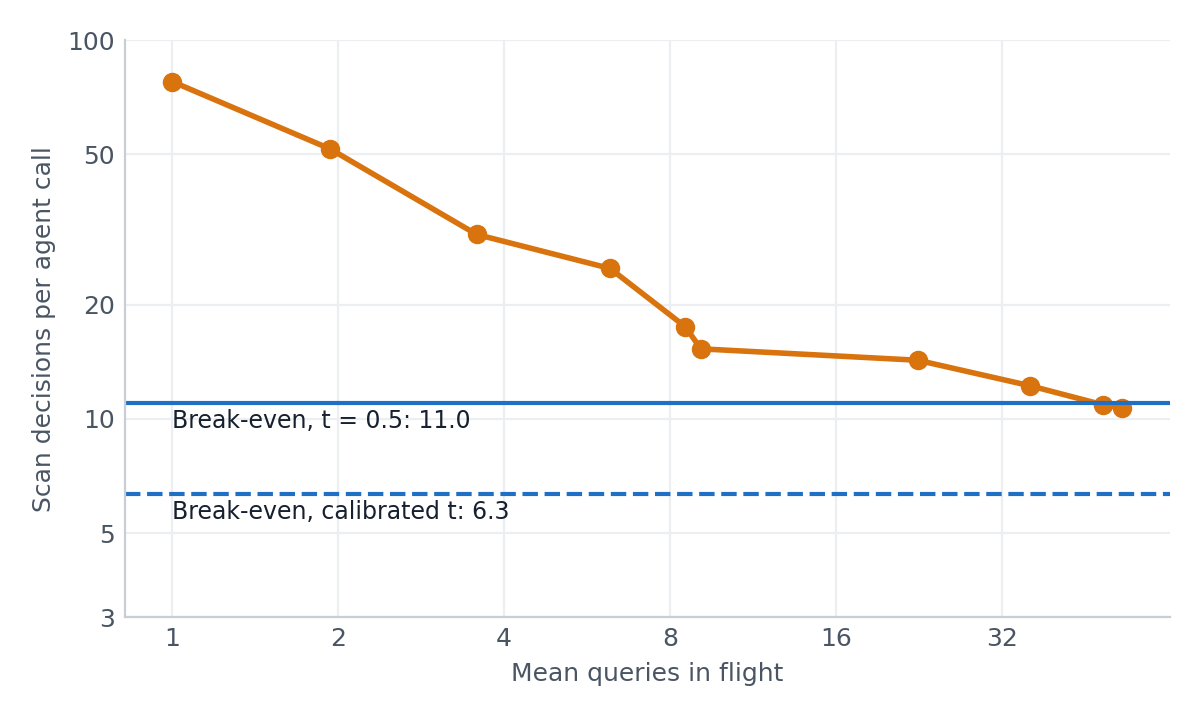
\includegraphics[width=0.62\linewidth]{exchange.png}
\caption{Exchange rate against the number of agent queries in flight
($N=10{,}000$). Lines mark the break-even rate $E^\ast$ at $t=0.5$ and at the
tuned threshold.}
\label{fig:exchange}
\end{figure}

The exchange rate is the same order across models but not the same number:
about 80--90 for Qwen2.5-1.5B and 122 for Phi-3.5-mini (210 documents per
second, 0.57\,s per call). However, the 1.5B and Phi agents stop after 1 to 1.5
searches, so only the 7B agent really searches, and our agent comparison rests
on that one model.

\subsection{Equal time: the ordered scan beats the agent}
\label{sec:equaltime}

Give the scan exactly the agent's time per query and let it classify documents
in embedding order. At $N=10{,}000$ the agent's 5.0\,s buys $k=849$ decisions,
which reach recall 0.256 against the agent's 0.087 (+0.168\ci{0.112}{0.232},
better on 19 of 20 queries), at precision 0.79 against 0.73
(Figure~\ref{fig:frontier}). The gap is +0.142 at $N=5{,}000$ and not
significant at $N=1{,}000$ (+0.048\ci{-0.003}{0.099}). The break-even rate is
$E^\ast = 11.0$ at $t=0.5$ and 6.3 at the tuned threshold.

One at a time, then, $E = 78 \gg E^\ast$ and the scan wins. With about 50
queries in flight, $E \approx 11 \approx E^\ast$: the batched agent ties the
scan ($+0.003$\ci{-0.019}{0.026}), but only at its own recall of 0.09, and with
the tuned threshold the scan still leads ($+0.060$\ci{0.038}{0.083}, 17 of 20).
Batching makes the agent cheaper, not more complete. Beyond the agent's
recall, the scan is the only arm that gets there.

\begin{figure}[t]
\centering
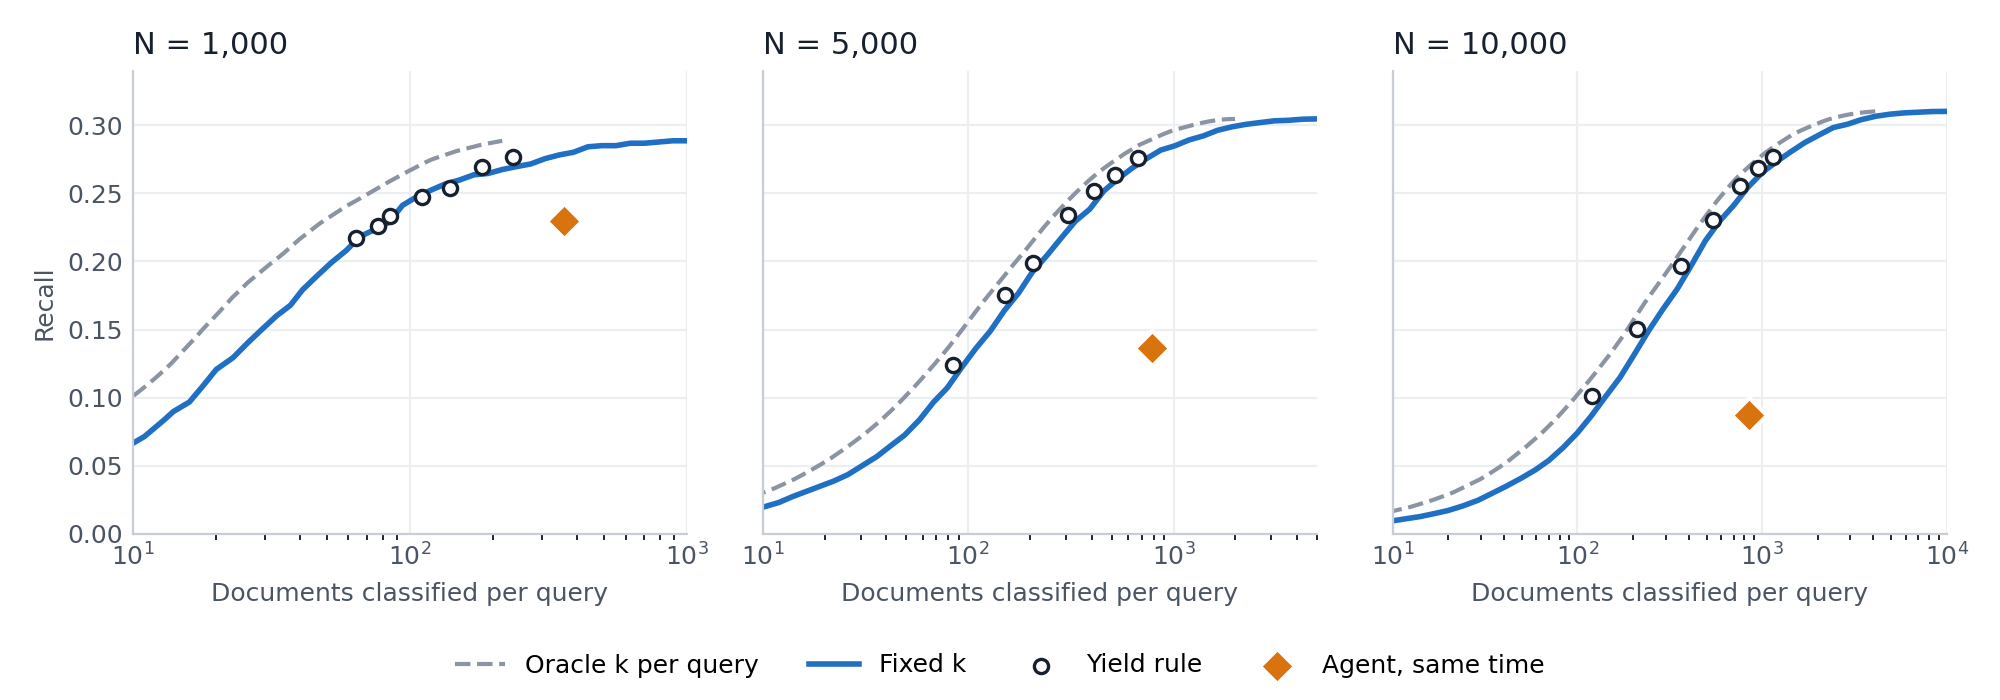
\includegraphics[width=\linewidth]{frontier.png}
\caption{Recall against documents classified per query, on 20 Newsgroups with
Qwen2.5-7B ($t=0.5$). Fixed $k$, the yield rule and the oracle all walk the
embedding ranking; the diamond is the agent at the scan depth its own time
would buy.}
\label{fig:frontier}
\end{figure}

On NFCorpus the scan is slower (95 documents per second, so $E$ falls from 33
to 3.7 when batched), and the agent passes the scan on recall only at 84
queries in flight (0.15 against 0.11), not on F1. That is one run, and the
agent's recall was 0.12--0.13 in four others, so we read it as noise as much as
a crossover.

\subsection{Adaptive $k$ does not beat fixed $k$}
\label{sec:adaptive}

A hybrid plan chooses an access path: how many documents to classify for this
query. We tested four rules that set $k$ per query, each compared with a fixed
$k$ at the same mean cost: \emph{mass} (documents whose similarity exceeds the
mean by $z$ standard deviations), \emph{gap} (the largest drop in similarity,
plus a buffer, after~\cite{taguchi2025adaptivek}), \emph{sample} (classify 200
random documents, estimate the answer size and set $k$ from it) and
\emph{yield} (classify in chunks of 32 and stop when the acceptance rate over
the last 64 falls below $y$).

None beats fixed $k$. Mass, gap and yield tie it, and sample loses. To see
whether any rule could do better, we computed a budget-optimal oracle that
knows the answers and spends a total budget across queries along each query's
concave hull. It adds only 0.01--0.04 recall over fixed $k$ on 20 Newsgroups
(Figure~\ref{fig:frontier}), where answer sizes barely vary (329--555), so $k$
has to follow $N$ rather than the query. The logic queries, whose answer sizes
span 18 to 1,046, leave more room (up to 0.07), but the rules still only tie
fixed $k$. NFCorpus has headroom at small budgets (0.14 to 0.18 at about 65
documents), which no rule reaches. This matches Meng et al.~\cite{meng2024rlt}.

Deployment needs a setting that transfers. We tuned each rule to reach 80\% of
the scan's recall on one corpus and applied it unchanged to another
(Table~\ref{tab:transfer}). A share of $N$ works within a corpus, but only the
yield rule reached 80\% in both directions across datasets. That is four pairs,
so we treat it as a lead, not a result.

\begin{table}[t]
\centering
\small
\begin{tabular}{@{}lrrr@{}}
\toprule
Tuned on $\rightarrow$ applied to & Fixed $k$ & $k$ as a share of $N$ & Yield \\
\midrule
20NG 1K $\rightarrow$ 20NG 10K & 0.21 & \textbf{0.83} & 0.63 \\
20NG 10K $\rightarrow$ NFCorpus & 0.95 & 0.92 & 0.80 \\
NFCorpus $\rightarrow$ 20NG 10K & 0.28 & 0.56 & \textbf{0.82} \\
\bottomrule
\end{tabular}
\caption{Share of the scan's recall reached when a setting tuned for 80\% on
one corpus is applied to another ($t=0.5$).}
\label{tab:transfer}
\end{table}

\subsection{Threshold and query shape}
\label{sec:threshold}

The zero-shot classifier ranks well but is extremely sure of ``no'': 97\% of
its scores are below 0.001. Its recall@100 at $N=1{,}000$ is 0.75 against 0.62
for embedding search, better on 19 of 20 queries, so the problem is the cut-off,
not the ranking. Tuned by leave-one-query-out, the threshold on 20 Newsgroups is
about $10^{-8}$; at $N=10{,}000$ that takes recall from 0.31 to 0.63, precision
from 0.76 to 0.59 and F1 from 0.42 to 0.58 (+0.16\ci{0.11}{0.21}). The choice is
stable, since only 0.09\% of decisions change between batch sizes 1 and 32. But
it does not transfer: NFCorpus prefers 0.9, and $10^{-8}$ there gives F1 0.06.

Query shape explains much of this (Table~\ref{tab:shape}). Narrow, exact
queries (keyword, AND) do best near 0.5, while broad topic queries (OR, NOT,
categories) want about $10^{-8}$, where NOT reaches recall 0.51. So one global
threshold is wrong for a zero-shot model. Keyword answer sets come from exact
word matches, so a plain text search would score 1.0 on them; they measure how
reliable the model is, not a reason to use one.

\begin{table}[t]
\centering
\small
\begin{tabular}{@{}lrrrr@{}}
\toprule
Shape (queries) & Scan recall & Scan precision & Agent recall & Agent precision \\
\midrule
Keyword (10) & 0.82 & 0.69 & 0.26 & 0.67 \\
AND (6) & 0.72 & 0.59 & 0.24 & 0.62 \\
OR (5) & 0.32 & 0.88 & 0.06 & 0.88 \\
NOT (4) & 0.10 & 0.74 & 0.06 & 0.63 \\
\bottomrule
\end{tabular}
\caption{Qwen2.5-7B scan and agent by query shape on the logic queries,
$N=10{,}000$, $t=0.5$.}
\label{tab:shape}
\end{table}

\subsection{Purpose-built decision models}
\label{sec:decision}

Table~\ref{tab:decision} replaces the zero-shot classifier with the open
decision models on the same documents. \todo{add JEV-9B columns.}

\begin{table}[t]
\centering
\small
\begin{tabular}{@{}lrrrrr@{}}
\toprule
& \multicolumn{2}{c}{F1 at $t=0.5$} & \multicolumn{2}{c}{F1, tuned $t$} & Kev $-$ Qwen \\
\cmidrule(lr){2-3}\cmidrule(lr){4-5}
Setting & Qwen & Kev & Qwen & Kev & (tuned) \\
\midrule
20NG 1K & 0.40 & 0.63 & 0.56 & 0.63 & +0.07\ci{0.04}{0.10} \\
20NG 5K & 0.41 & 0.64 & 0.58 & 0.65 & +0.07\ci{0.04}{0.10} \\
20NG 10K & 0.42 & 0.64 & 0.58 & 0.65 & +0.07\ci{0.04}{0.11} \\
NFCorpus & 0.12 & 0.15 & 0.12 & 0.18 & +0.06\ci{0.02}{0.10} \\
Logic 1K & 0.59 & 0.73 & 0.57 & 0.76 & +0.19\ci{0.12}{0.25} \\
Logic 10K & 0.56 & 0.70 & 0.58 & 0.77 & +0.19\ci{0.15}{0.23} \\
\bottomrule
\end{tabular}
\caption{Zero-shot Qwen2.5-7B against Kev-9B as the scan's classifier. The
tuned threshold is chosen by leave-one-query-out; the last column is the paired
difference with a 95\% bootstrap interval.}
\label{tab:decision}
\end{table}

\paragraph{Recall without tuning.}
At $t=0.5$, Kev's recall at $N=10{,}000$ is 0.78, against 0.31 for Qwen; Qwen
needs $t=10^{-8}$ to reach 0.63. Kev's tuned threshold is between 0.5 and 0.9
in every setting, so the threshold problem of \S\ref{sec:threshold} is a
property of the zero-shot model, not of scanning.

\paragraph{Query shape.}
At $N=10{,}000$ and $t=0.5$, Kev's F1 is 0.74 (keyword), 0.54 (AND), 0.79 (OR)
and 0.70 (NOT), against Qwen's 0.73, 0.63, 0.45 and 0.18. NOT recall rises from
0.10 to 0.78. Kev is behind only on AND at 0.5, where it accepts too much
(precision 0.40); with a tuned threshold it leads there too (0.78 against 0.58).

\paragraph{Equal time against the agent.}
Table~\ref{tab:kevtime} repeats the equal-time comparison with Kev as the scan.
One query at a time, Kev scores 121 documents per second, slower than Qwen's
170, yet it beats the agent on every query at every size. Packed, it scores
540 documents per second per query, but only when the queries arrive together,
so it suits batch workloads rather than one-off questions. In exchange-rate
terms, one Qwen agent step buys about 56 Kev decisions one at a time, or about
250 packed.

\begin{table}[t]
\centering
\small
\begin{tabular}{@{}rrrrr@{}}
\toprule
$N$ & Agent & Qwen scan & Kev, separate & Kev, packed \\
\midrule
1,000 & 0.23 & 0.28 & 0.68 & 0.77 (all) \\
5,000 & 0.14 & 0.28 & 0.59 & 0.75 \\
10,000 & 0.09 & 0.26 & 0.48 & 0.71 \\
\bottomrule
\end{tabular}
\caption{Recall in the agent's own time per query, scanning in embedding order
($t=0.5$). Kev beats the agent on all 20 queries at every size.
\todo{add JEV-9B column.}}
\label{tab:kevtime}
\end{table}

\paragraph{Hybrid and NFCorpus.}
Classifying the top 1,000 by embedding at $N=10{,}000$ gives recall 0.57 with
Kev against 0.27 with Qwen. NFCorpus remains hard: Kev is the best arm there
(tuned F1 0.18, against 0.15 for Qwen's hybrid and 0.12 for the agent), but its
recall does not improve (0.19 for both models at the tuned threshold).

\paragraph{Calibration.}
Kev is not better calibrated. Its expected calibration error is 0.06 against
0.04 for Qwen, and above 0.5 it predicts 0.81 on average while being right about
half the time. Qwen errs the other way, with nearly all scores near 0 or 1.

\todo{JEV-9B paragraph: accuracy, throughput, calibration, and whether it
agrees with Kev.}

% ---------------------------------------------------------------------------
\section{Discussion}

\paragraph{When to scan and when to search.}
The exchange rate turns the question into arithmetic. If one agent step costs
more scan decisions than the agent's depth-per-step at break-even
($E > E^\ast$), scanning in embedding order is better at equal time, and the
scan can keep going to recall levels the agent never reaches. On one GPU with
queries arriving one at a time, $E$ is far above $E^\ast$. Many agents sharing
a GPU bring $E$ down to $E^\ast$, but only buy parity at the agent's own recall,
at about 20 times the latency. An agent is the right choice when only a few
answers are needed quickly; when the answer set must be complete, the scan is
the only arm that gets there, and a decision model makes it far better.

\paragraph{Is the comparison fair?}
The agent and the hybrid are not exhaustive and are not meant to be. Every arm
is scored against the full answer set, so a missed document always counts as
lost recall, and arms are compared at equal cost rather than equal effort.
The agent's only tool is top-$k$ embedding search with paging; richer tools
(keyword search, metadata filters, or a tool that runs the classifier on a
batch) might help it, but a top-$k$ loop that stops when results dry up is
exactly what the agent already does, and it still misses most answers.

\paragraph{Limitations.}
The agent comparison rests on one model that really searches (Qwen2.5-7B);
smaller agents barely search. 20 Newsgroups has 20 category queries with large
answer sets, and the logic set has only 4--10 queries per shape. All timing is
on one GPU type. Kev and JEV-9B use a different and larger backbone than Qwen,
so the decision-model results compare models, not only architectures. Packed
throughput depends on how many queries share a pass. NFCorpus judgments are
incomplete, so its recall numbers are a lower bound on quality.

\paragraph{Future work.}
Query rewriting, where a strong model decomposes the request once and a cheap
model executes it $N$ times; LOTUS-style cascades~\cite{patel2024lotus,
kim2026semfilter} with a decision model as the oracle; agents with richer
tools; and corpora that change, where the scan must be rerun on every update
while an index amortises.

% ---------------------------------------------------------------------------
\section{Conclusion}

For find-all queries, scanning beats searching whenever an agent step costs
more than a handful of classifier decisions, which on one GPU it does by a
factor of seven. Batching agents closes the cost gap but not the recall gap.
Choosing scan depth per query buys little over a fixed depth. And the scan's
weakness in our first experiments, low recall from a zero-shot model, largely
disappears with an open decision model built for the job.

\paragraph{Reproducibility.}
Code, submit files, raw rows and per-document scores are in the project
repository. \texttt{src.access\_paths}, \texttt{src.crossover} and
\texttt{src.kev\_compare} regenerate every replayed number from the saved
scores without a GPU.

\bibliographystyle{plainnat}
\bibliography{refs}

\end{document}
